% !TEX root = ../main.tex
% \section{Preliminaries}\label{sec:prelim}

% % \subsection{Path decomposition}
% \subsection{Basic definitions}
% \begin{definition}[Path Decomposition \cite{cygan2015parameterized}]\label{def:path_dec}
% A \textit{path decomposition} of a graph $G = (V, E)$ is a sequence of bags $\mathcal{P} = \{X_1, \dots, X_r\}$, where each $X_i \subseteq V$ such that following conditions hold:
% \begin{enumerate}
% 	\item For each $v \in V$, there exists a pair of indices 
% 	$1 \leq l(v) \leq r(v) \leq r$ such that 
% 	\[v \in X_i \Longleftrightarrow l(v) \leq i \leq r(v).\]
% 	In other words each graph vertex maps to continuous subpath of the decomposition.   
% 	\item For each $uv \in E$, there exists an $i$ such that $\{u, v \} \subseteq X_i$.
% \end{enumerate}

% \end{definition}
% \begin{definition}[Nice Path Decomposition \cite{cygan2015parameterized}]\label{def:nice_path_dec}
% A \textit{nice path decomposition} is a path decomposition, where additional conditions hold:
% \begin{enumerate}
% 	\item $X_1, X_r = \varnothing$.
% 	\item Each bag, except $X_1$, either \textit{introduce} or \textit{forget} node.
% 	\item If $X_{i + 1}$ is a forget node, then there exists $v \in V$ such that $X_{i + 1} = X_i \setminus \{v\}$.
% 	\item  If $X_{i + 1}$ is an introduce node, then there exists $v \in V$ such that $X_{i + 1} = X_i \cup \{v\}$.
	
% \end{enumerate}
% \end{definition}

% \begin{definition}[Pathwidth \cite{cygan2015parameterized}]\label{def:pathwidth}
% The width of a path decomposition $\mathcal{P} = \{X_1, \dots, X_r\}$ is $max_{1 \leq i \leq r} \lvert X_i \rvert - 1$. The pathwidth of a graph $G$, denoted by pw(G), is the minimum possible width of a path decomposition
% of G.
% \end{definition}



% \begin{definition}[Tree Decomposition \cite{cygan2015parameterized}]\label{def:tree_dec} 
% A \textit{tree decomposition} of a graph $G$ is a pair $\mathcal{T} = (T, \{X_t\}_{t \in V(T)})$, where $T$ is a rooted tree with a root $r$, each bag $X_t \subseteq V(G)$ and the following conditions hold:
% \begin{enumerate}
% 	\item For every $uv \in E(G)$, there exists a node $t \in V(T)$ such that $\{u, v\} \subseteq X_t$.
% 	\item For every $v \in V(G)$, the set $T_v := \{t \in V(T): v \in X_t\}$, induced graph $T[T_v]$ is nonempty subtree of the $T$. 
% \end{enumerate}
% \end{definition}


% \begin{definition}[Nice Tree Decomposition \cite{cygan2015parameterized}]\label{def:nice_tree_dec}
% A \textit{nice tree decomposition} is a tree decomposition, where additional conditions hold:

% \begin{enumerate}
% 	\item The root bag is empty: $X_r = \varnothing$.
% 	\item If $l$ is a leaf of the $T$, then $X_l = \varnothing$.
% 	\item Each non-leaf node of tree $T$ is of one of the three types: \textit{introduce}, \textit{forget} or \textit{join} node.
% 	\item If $X_b$ is a forget node, it has exactly one child $X_c$ and there is a vertex $v \in X_c$ such that $X_b = X_c \setminus \{v\}$.
% 	\item If $X_b$ is an introduce node, it has exactly one child $X_c$ and there is a vertex $v \in V(G) \setminus X_c$ such that $X_b = X_c \cup \{v\}$.
% 	\item If $X_b$ is a join node, it has exactly two children $X_{c_1}$ and $X_{c_2}$ such that $X_b = X_{c_1} = X_{c_2}$. 
% \end{enumerate}
% \end{definition}

% \begin{definition}[Treewidth \cite{cygan2015parameterized}]\label{def:treewidth}
% The width of tree decomposition $\mathcal{T} = (T, \{X_t\}_{t \in V(T)})$ equals $max_{t \in V(T)} \lvert X_t \rvert - 1$, that is, the maximum size of its bag minus 1. The treewidth of a graph $G$, denoted by $tw(G)$, is the minimum possible width of a tree decomposition of $G$.
% \end{definition}

% \begin{remark}
% Notice that (nice) path decomposition is a special case of a (nice) tree decomposition. For a path decomposition $\mathcal{P} = \{X_1, \dots, X_r\}$ we think that the $X_1$ is a leaf bag and the $X_r$ is a root bag. 
% \end{remark}



% \begin{notation}\label{notation:subtree}
% For each $t \in G(T)$ we denote subtree rooted at this vertex as $T_t$, and denote a graph induced by all vertices in all bags correspond to $T_t$:
% \[
% G^\downarrow_t := G\left[\bigcup \{X_t: t \in T_t\}\right].
% \]
% \end{notation}

% \begin{example}\label{example:explaining_tree_decomposition}
% 	In this example, we explain the above defintions by explicitly showing tree decomposition for underlying graph of Caffeine molecule (See Figure \ref{fig:caffeine example}).
% 	\begin{figure}[H]
% 		\centering
% 		\chemfig{O=[:270]-[:210]N(-[:150])-[:270](=[:210]O)-[:330]N(-[:270])-[:30]%
-[:342.2,0.994]N=^[:54,0.994]-[:126,0.994]N(-[:71.9])-[:197.8,0.994](%
=^[:270])(-[:150])}

% 		\caption{Caffeine}
% 		\label{fig:caffeine example}
% 	\end{figure}

% 	We can see from Figure \ref{fig:tree_dec_caffeine}, that Caffeine molecule has treewidth $2$.

% 	% See Figure \ref{fig:caffeine example} for Caffeine, it has treewidth $2$.

% 	\begin{figure}[H]
% 		\centering
% 		\subfloat[][Graph of Caffeine]{\resizebox{0.25\textwidth}{!}{% \begin{center}
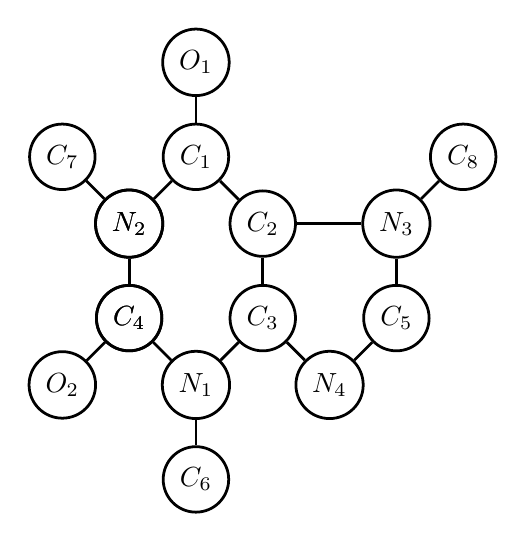
\begin{tikzpicture}[node distance={12mm}, line width=1pt, main/.style = {draw, circle}] 
\node[main] (1) []{$C_1$}; 
\node[main] (2) [below right of=1]{$C_2$}; 
\node[main] (3) [below of=2]{$C_3$}; 
\node[main] (4) [below left of=3]{$N_1$}; 
\node[main] (5) [above left of=4]{$C_4$}; 
\node[main] (6) [above of=5]{$N_2$};
\node[main] (9) [below right of=3]{$N_4$}; 
\node[main] (8) [above right of=9]{$C_5$}; 
\node[main] (7) [above of=8]{$N_3$}; 
\node[main] (10) [above of=1]{$O_1$}; 
\node[main] (11) [above left of=4]{$C_4$}; 
\node[main] (12) [above of=5]{$N_2$}; 

\node[main] (13) [below of=4]{$C_6$};  

\node[main] (17) [below left of=5]{$O_2$};

\node[main] (18) [above left of=6]{$C_7$}; 

\node[main] (22) [above right of=7]{$C_8$}; 



\draw [] (1) -- (2); 
\draw [] (2) -- (3); 
\draw [] (3) -- (4); 
\draw [] (4) -- (5); 
\draw [] (5) -- (6); 
\draw [] (6) -- (1); 
\draw [] (2) -- (7); 
\draw [] (7) -- (8); 
\draw [] (8) -- (9); 
\draw [] (9) -- (3); 
\draw [] (1) -- (10); 

\draw [] (4) -- (13); 

\draw [] (5) -- (17); 

\draw [] (6) -- (18); 

\draw [] (7) -- (22); 
\end{tikzpicture}
% \end{center}
}}
% 		\qquad
% 		\qquad
% 		\qquad
% 		\qquad
% 		\subfloat[][Tree decomposition]{\resizebox{0.35\textwidth}{!}{% \begin{center}
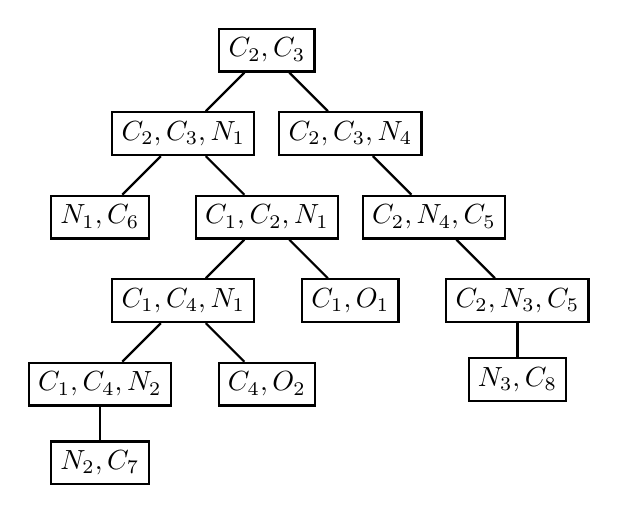
\begin{tikzpicture}[node distance={15mm}, thick, main/.style = {draw, rectangle}] 
\node[main] (0) []{$C_2,C_3$}; 
\node[main] (00) [below left of =0]{$C_2,C_3,N_1$};
\node[main] (000) [below left of =00]{$N_1,C_6$};
\node[main] (001) [below right of =00]{$C_1,C_2,N_1$};
\node[main] (0011) [below right of =001]{$C_1,O_1$};
\node[main] (0010) [below left of =001]{$C_1,C_4,N_1$};
\node[main] (00101) [below right of =0010]{$C_4,O_2$};
\node[main] (00100) [below left of =0010]{$C_1,C_4,N_2$};
\node[main] (001000) [below of =00100,,node distance={10mm}]{$N_2,C_7$};
\node[main] (01) [below right of =0]{$C_2,C_3,N_4$};
\node[main] (011) [below right of =01]{$C_2,N_4,C_5$};
\node[main] (0111) [below right of =011]{$C_2,N_3,C_5$};
\node[main] (01110) [below of =0111,,node distance={10mm}]{$N_3,C_8$};

\draw [] (0) -- (00); 
\draw [] (00) -- (000); 
\draw [] (00) -- (001); 
\draw [] (001) -- (0010); 
\draw [] (001) -- (0011); 
\draw [] (0010) -- (00100); 
\draw [] (00100) -- (001000);  
\draw [] (0010) -- (00101); 

\draw [] (0) -- (01); 
\draw [] (01) -- (011); 
\draw [] (011) -- (0111); 
\draw [] (0111) -- (01110); 

\end{tikzpicture}
% \end{center}}}
% 		\caption{Graph representation and tree decomposition of Caffeine. Nodes on the root bag of the tree decomposition are highlighted in green (dashed). Notice how the removal of these nodes in the original molecule separates it into two connected components, each corresponding to one of the highlighted subtrees in the tree decomposition.}
% 		\label{fig:tree_dec_caffeine}
% 	\end{figure}


% \end{example}
% % \begin{figure}[H]
% % 	\centering
% % 	\chemfig{=^[:270](-[:330]=^[:30]-[:90]=^[:150]-[:210])-[:210]=_[:270](%
-[:330]=_[:30]-[:330]=_[:270]-[:210]=_[:150]-[:90])-[:210](-[:270]=_[:330]%
-[:270]=_[:210]-[:150]=_[:90]-[:30])=_[:150](-[:210]=_[:270]-[:210]=_[:150]%
-[:90]=_[:30]-[:330])-[:90](-[:150]=^[:90]-[:150]=^[:210]-[:270]=^[:330]%
-[:30])=_[:30](-[:330])-[:90]=^[:30]-[:90]=^[:150]-[:210]=^[:270](-[:330])}

% % 	\caption{1,2,3,4,5,6-hexakis-phenylbenzene}
% % 	\label{fig:tw_2 example}
% % \end{figure}


% \subsection{Technical Lemmas}
% \noindent We now present two technical lemmas that are crucial for development of algorithms in Section \ref{sec:algos}. These lemmas are consequences of separation properties of the tree decomposition.

% \begin{lemma}[Proof in Appendix~\ref{appendix:proof_intseplemma}]\label{intseplemma}
% 	If $X_b$ is an introduce nodes, $X_b = X_c \cup \{v\}$, then $N(v)\cap G_b^\downarrow \subseteq X_c$.
% \end{lemma}
% % \begin{proof} 
% % Let $T^\prime$ be a subtree of the tree $T$ rooted at $b$. Observe that the corresponding tree decomposition
% % $\mathcal{T}^\prime = \{T^\prime, \{X_t\}_{t\in V(T^\prime)}\}$ is a tree decomposition of $G_b^\downarrow$. Notice that by Definition \ref{def:tree_dec}, $T^\prime_v$ forms an induced subtree of the $T^\prime$. As $v \notin X_c$ and $c$ is the only vertex in the open neighbourhood of $b$, this implies that $T^\prime_v = \{b\}$.

% % Let $u$ be a vertex in $N(v) \cap G_b^\downarrow$, then by Definition \ref{def:tree_dec}, if there is an edge $uv$ in $G_b^\downarrow$, then there exists a bag containing both $u$ and $v$. But, as we have just shown that the only bag containing $v$ is $X_b$. As $u$ is a vertex in $N(v)$, this implies that $u \in X_c$.
% % \end{proof}
% \begin{lemma}[Proof in Appendix~\ref{appendix:proof_joinseplemma}]\label{joinseplemma}
% 	If $X_b$ is a join node with two children $X_b = X_{c_1} = X_{c_2}$, then in $G_b^\downarrow$ there is no edge between $V(G_{c_1}^\downarrow) \setminus X_b$ and $V(G_{c_2}^\downarrow) \setminus X_b$.
% \end{lemma}
% % \begin{proof}
% % Let $T^\prime, T^{\prime\prime}, T^{\prime\prime\prime}$ be the subtrees of $T$ rooted at $b, c_1, c_2$ respectively. Let 
% % $\mathcal{T}^\prime, \mathcal{T}^{\prime\prime}, \mathcal{T}^{\prime\prime\prime}$ be the corresponding tree decompositions. We will prove the given statement by contradiction. Therefore, let us assume that $u \in V(G_{c_1}^\downarrow) \setminus X_b$, $v \in V(G_{c_2}^\downarrow) \setminus X_b$, and $uv \in E(G_b^\downarrow)$.

% % As $\mathcal{T}^{\prime}$ is a tree decomposition of $G^\downarrow_b$, there exists at least one bag $X_t$, such that $t \in \mathcal{T}^{\prime}$ and $u,v \in X_t$. From our initial assumption, we know that $u, v \notin X_b$, this implies that $t \neq b$. Therefore, either $t \in T^{\prime\prime}$ or $t \in T^{\prime\prime\prime}$. Without loss of generality, let us assume that $t \in T^{\prime\prime}$. As $v \in V(G_{c_2}^\downarrow) \setminus X_b$, there exists at least one bag $X_s$ such that, $ s \in T^{\prime\prime\prime}$ and $v \in X_s$. Observe that $v$ appears in both bags $X_s$ and $X_t$. Now by Definition \ref{def:tree_dec}, we know that $T^\prime_{v}$ is a connected subtree and any path connecting $s$ and $t$ goes through $b$. This implies that $X_b \in T^\prime_v$ and $v \in X_b$. This contradicts our initial assumption that $v \notin X_b$, hence completes the proof.
% % \end{proof}
 
\section{Our Algorithms}\label{sec:algos} 
%\subsection{Counting Perfect Matchings}\label{sec:perfect_matchings}
%Enumeration of Kekulé structures in organic molecules is equivalent to finding total number of perfect matchings for the underlying chemical graph of the molecule.
%
%We present parameterized algorithms for the cases when the underlying chemical graph have bounded pathwidth and bounded treewidth respectively.

We now present our algorithms. We assume that the input contains a graph $G,$ modeling a molecule, as well as a nice decomposition of $G.$ This is without loss of generality since there are linear-time FPT algorithms parameterized by the treewidth/pathwidth to compute optimal tree/path decompositions~\cite{bodlaender1996efficient,DBLP:journals/siamcomp/Bodlaender96}. Moreover, the decompositions can also be made nice in linear time~\cite{cygan2015parameterized}. In each case, we first provide an algorithm for nice path decompositions, i.e.~handling introduce and forget nodes, and then extend it to nice tree decompositions by adding extra steps for join nodes.
Due to space restrictions and the similarity among algorithms, we have relegated most cases to~\ref{sec:remalgo}. Figures illustrating the algorithms are presented in~\ref{app:fig}.

\subsection{Counting Kekulé Structures / Perfect Matchings}\label{subsec:perfect_pathwidth}

% We present a dynamic programming approach over the given nice path decomposition.

\begin{definition}[Respectful Perfect Matchings]\label{def:respectful_perfect_matching}
Let $\mathcal{P} = \{X_1, \dots X_r\}$ be a nice path decomposition of $G.$ For each $b \in \{1, 2, \ldots, r\}$ and each $M \subseteq X_b$, we define $\RP(b,M)$ as the set of all perfect matchings $F$ in $G_b^\downarrow \setminus M$ such that each matching edge $uv \in F$ has at least one endpoint in $G_b^\downarrow \setminus X_b,$ i.e.~$u \notin X_b$ or $v \notin X_b$. We define $\pma[b, M] := |\RP(b,M)|.$
\end{definition}

\paragraph{Our Dynamic Programming Algorithm (Figures illustrating the algorithm steps are provided in \ref{appendix:figure_perfect_matching})} We note that since $X_r = \emptyset$ is the root node, $G_{r}^\downarrow = G$ and perfect matchings of $G$ are the same as respectful perfect matchings in $\RP(r,\emptyset).$ Thus $\pma [r, \emptyset]$ is the desired number of perfect matchings / Kekulé structures. We now provide a bottom-up dynamic programming approach to compute the $\pma[\cdot, \cdot]$ values. This is based on a case-work on the type of nodes:
\begin{compactitem}
\item \textbf{Leaves:} If $X_l$ is a leaf bag then $\RP(l,\emptyset)$ contains only the empty matching as $X_l = \emptyset.$ Therefore, $\pma[l,\emptyset]=1$.
\item \textbf{Introduce Nodes:} Let $b$ be a bag introducing $v$ and having a single child $c.$ We have
\[
\pma [b,M] =
\begin{cases}
\pma [c,M\setminus \{v\}] &v \in M\\
0 &v \not\in M
\end{cases}.
\]
In order to derive the above recurrence relations, we consider two possibilities for $v:$
\begin{compactenum}
\item If $v \in M$, then by Definition \ref{def:respectful_perfect_matching}, the matchings in $\RP(b,M)$ are the same as the matchings in $\RP(c, M \setminus \{v\})$. 
\item If $v \notin M$, then for every matching $F \in \RP(b,M)$, $v$ should be covered by some edge $vw \in F$. By Lemma \ref{intseplemma}, $w \in X_{c} \subset X_b$, which contradicts the requirements of Definition~\ref{def:respectful_perfect_matching}. Therefore, $\pma[b,M] = 0.$ %for this case, as there are no matchings satisfying the given conditions.
\end{compactenum}

% \begin{figure}[h]
% \floatbox[{\capbeside\thisfloatsetup{capbesideposition={right,top},capbesidewidth=7cm}}]{figure}[\FBwidth]
% {\caption{Computing values in introduce nodes. Each of the squares corresponds to a bag. In each case, bag $b$ introduces node $x_1$ and has child $c$. Nodes in red (dashed) represent $M$, i.e~nodes that are not yet ``matched''. In the left example, since $x_1\in M$, the number of respectful perfect matchings is $\pma [c,M\setminus \{x_1\}]$. In the example on the right, $x_1\not \in M$, i.e~$x_1$ should be matched with a node outside of $X_b$. This is not possible since $x_1$ has just been introduced, thus the number of respectful matchings is $0.$}\label{fig:introduce_node}}
% {\resizebox{0.35\textwidth}{!}{\begin{tikzpicture}[line width=1pt,node distance=14mm ,main/.style = {draw, rectangle},scale=1] 
    \node[scale=.8] at (0,5.5){$\textup{PerfMatch}[b,\{x_1,x_2,x_3,x_4\}]$};
   \node[main] at (0,4) (9) {
   \begin{tikzpicture}[line width=1pt,node distance=14mm ,main/.style = {draw, circle},scale=1] 
   \node[main,color=red, densely dashed] at (0,1) (x1) {\texttt{$x_1$}};
   \node[main,color=red,densely dashed] at (1,1) (x2) {\texttt{$x_2$}};
       \node[main,color=red,densely dashed] at (0,0) (x3) {\texttt{$x_3$}};
       \node[main,color=red,densely dashed] at (1,0) (x4) {\texttt{$x_4$}};
      \draw (x1) -- (x2);
       \draw (x1) -- (x3);
      \draw (x2) -- (x3);
      \draw (x3) -- (x4);
   \end{tikzpicture}
       };
   
    \node[scale=.8] at (3.5,5.5){$\textup{PerfMatch}[b,\{x_1,x_4\}]$};
       \node[main] at (3.5,4) (9) {
   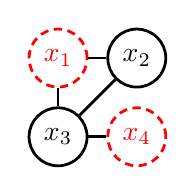
\begin{tikzpicture}[line width=1pt,node distance=14mm ,main/.style = {draw, circle},scale=1] 
   \node[main,color=red,densely dashed] at (0,1) (x1) {\texttt{$x_1$}};
   \node[main,color=black] at (1,1) (x2) {\texttt{$x_2$}};
       \node[main,color=black] at (0,0) (x3) {\texttt{$x_3$}};
       \node[main,color=red,densely dashed] at (1,0) (x4) {\texttt{$x_4$}};
      \draw (x1) -- (x2);
       \draw (x1) -- (x3);
      \draw (x2) -- (x3);
      \draw (x3) -- (x4);
   \end{tikzpicture}
       };
   
   \node[scale=.8] at (7,5.5){$\textup{PerfMatch}[b,\{x_1,x_2\}]$};
       \node[main] at (7,4) (9) {
   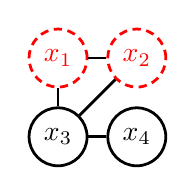
\begin{tikzpicture}[line width=1pt,node distance=14mm ,main/.style = {draw, circle},scale=1] 
   \node[main,color=red,densely dashed] at (0,1) (x1) {\texttt{$x_1$}};
   \node[main,color=red,densely dashed] at (1,1) (x2) {\texttt{$x_2$}};
       \node[main,color=black] at (0,0) (x3) {\texttt{$x_3$}};
       \node[main,color=black] at (1,0) (x4) {\texttt{$x_4$}};
      \draw (x1) -- (x2);
       \draw (x1) -- (x3);
      \draw (x2) -- (x3);
      \draw (x3) -- (x4);
   \end{tikzpicture}
       };
       
    \node[scale=.8] at (0,1.5){$\textup{PerfMatch}[c,\{x_2,x_3,x_4\}]$};
       \node[main] at (0,0) (8) {
   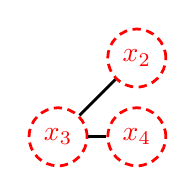
\begin{tikzpicture}[line width=1pt,node distance=14mm ,main/.style = {draw, circle},scale=1] 
   \node[main,color=red,densely dashed] at (1,1) (x2) {\texttt{$x_2$}};
       \node[main,color=red,densely dashed] at (0,0) (x3) {\texttt{$x_3$}};
       \node[main,color=red,densely dashed] at (1,0) (x4) {\texttt{$x_4$}};
      \draw (x2) -- (x3);
      \draw (x3) -- (x4);
   \end{tikzpicture}
   };
   
    \node[scale=.8] at (3.5,1.5){$\textup{PerfMatch}[c,\{x_4\}]$};
   \node[main] at (3.5,0) (8) {
   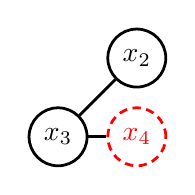
\begin{tikzpicture}[line width=1pt,node distance=14mm ,main/.style = {draw, circle},scale=1] 
   \node[main,color=black] at (1,1) (x2) {\texttt{$x_2$}};
       \node[main,color=black] at (0,0) (x3) {\texttt{$x_3$}};
       \node[main,color=red,densely dashed] at (1,0) (x4) {\texttt{$x_4$}};
      \draw (x2) -- (x3);
      \draw (x3) -- (x4);
   \end{tikzpicture}
   };
   
    \node[scale=.8] at (7,1.5){$\textup{PerfMatch}[c,\{x_2\}]$};
   \node[main] at (7,0) (8) {
   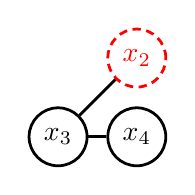
\begin{tikzpicture}[line width=1pt,node distance=14mm ,main/.style = {draw, circle},scale=1] 
   \node[main,color=red,densely dashed] at (1,1) (x2) {\texttt{$x_2$}};
       \node[main,color=black] at (0,0) (x3) {\texttt{$x_3$}};
       \node[main,color=black] at (1,0) (x4) {\texttt{$x_4$}};
      \draw (x2) -- (x3);
      \draw (x3) -- (x4);
   \end{tikzpicture}
   };
   
   
   
       \draw [->](0,2) -- (0,2.5);
       \draw [->](3.5,2) -- (3.5,2.5);
       \draw [->](7,2) -- (7,2.5);
   
   
    \node[scale=.8] at (10.5,5.5){$\textup{PerfMatch}[b,\{x_3,x_4\}]$};
       \node[main] at (10.5,4) (9) {
   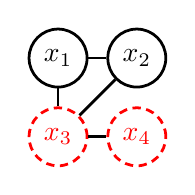
\begin{tikzpicture}[line width=1pt,node distance=14mm ,main/.style = {draw, circle},scale=1] 
   \node[main,color=black] at (0,1) (x1) {\texttt{$x_1$}};
   \node[main,color=black] at (1,1) (x2) {\texttt{$x_2$}};
       \node[main,color=red,densely dashed] at (0,0) (x3) {\texttt{$x_3$}};
       \node[main,color=red,densely dashed] at (1,0) (x4) {\texttt{$x_4$}};
      \draw (x1) -- (x2);
       \draw (x1) -- (x3);
      \draw (x2) -- (x3);
      \draw (x3) -- (x4);
   \end{tikzpicture}
       };
   
       \draw [->](10.5,1) -- (10.5,2.5);
       \node[scale=3] at (10.5,0){$\varnothing$};
       %\node[text width=6cm] at (2,-2){$\DP[i,c]$};
       %\node[text width=6cm] at (5.5,-2){$\DP[i,c+\{x_4\to \texttt{gray/dotted}]$};
      
   \end{tikzpicture}
   }}
% \end{figure}

\item \textbf{Forget Nodes:} Let $b$ be a forget node with a single child $c$ and $X_b = X_c \setminus \{v\}$. We have:
\[
\pma[b,M]=
	\textstyle	\pma[c, M] + \sum_{u \in X_b\setminus M:\ uv\in E(G)}\pma[c, M \cup \{u, v\}].
\]

To see this, consider a matching $F \in \RP(b, M).$ This matching must match the forgotten vertex $v$ with another vertex $u.$ We consider two cases: (i)~the matchings for which $u \not\in X_b$ are the same as those in $\RP(c, M);$ and (ii)~the matchings $F$ for which $u \in X_b$ are counted by the sum. Here, since $v$ is matched to $u,$ neither need to be further matched in $G^\downarrow_c.$

% \begin{figure}[h]
% \floatbox[{\capbeside\thisfloatsetup{capbesideposition={right,top},capbesidewidth=5cm}}]{figure}[\FBwidth]
% {\caption{Computing values in forget nodes. Bag $b$ forgets node $x_1$ and has child $c$. Notice that nodes $x_2$ and $x_3$ have been matched with some element not in $X_b$. Since we consider a perfect matching, $x_1$ must have been matched before being forgotten. We thus consider the cases where $x_1$ was already matched in $c$, where $x_1$ matched with $x_2$ and where $x_1$ matched with $x_3$.
% }\label{fig:forget_node}}
% {\resizebox{0.58\textwidth}{!}{% !TEX root = ../main.tex
\begin{tikzpicture}[line width=1pt,node distance=14mm ,main/.style = {draw, rectangle},scale=1] 

    \node[scale=.8] at (3,6){$\textup{PerfMatch}[b,\{x_4\}]$};
       
       \node[main] at (3,4.5) (9) {
   \begin{tikzpicture}[line width=1pt,node distance=14mm ,main/.style = {draw, circle},scale=1] 
   \node[main,color=black] at (1,1) (x2) {\texttt{$x_2$}};
       \node[main,color=black] at (0,0) (x3) {\texttt{$x_3$}};
       \node[main,fill=red!40!white,densely dashed] at (1,0) (x4) {\texttt{$x_4$}};
      \draw (x2) -- (x3);
      \draw (x3) -- (x4);
   \end{tikzpicture}
       };
       
    \node[scale=.8] at (-1,1.5){$\textup{PerfMatch}[c,\{x_4\}]$};
       \node[main] at (-1,0) (8) {
   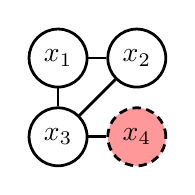
\begin{tikzpicture}[line width=1pt,node distance=14mm ,main/.style = {draw, circle},scale=1] 
   \node[main,color=black] at (0,1) (x1) {\texttt{$x_1$}};
   \node[main,color=black] at (1,1) (x2) {\texttt{$x_2$}};
       \node[main,color=black] at (0,0) (x3) {\texttt{$x_3$}};
       \node[main,fill=red!40!white,densely dashed] at (1,0) (x4) {\texttt{$x_4$}};
      \draw (x1) -- (x2);
       \draw (x1) -- (x3);
      \draw (x2) -- (x3);
      \draw (x3) -- (x4);
   \end{tikzpicture}
   };
   
    \node[scale=.8] at (3,1.5){$\textup{PerfMatch}[c,\{x_4\}\cup \{x_1,x_2\}]$};
   \node[main] at (3,0) (8) {
   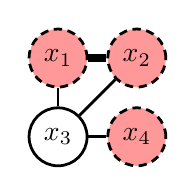
\begin{tikzpicture}[line width=1pt,node distance=14mm ,main/.style = {draw, circle},scale=1] 
   \node[main,fill=red!40!white,densely dashed] at (0,1) (x1) {\texttt{$x_1$}};
   \node[main,fill=red!40!white,densely dashed] at (1,1) (x2) {\texttt{$x_2$}};
       \node[main,color=black] at (0,0) (x3) {\texttt{$x_3$}};
       \node[main,fill=red!40!white,densely dashed] at (1,0) (x4) {\texttt{$x_4$}};
      \draw [line width = 3pt, color=black]  (x1) -- (x2);
       \draw (x1) -- (x3);
      \draw (x2) -- (x3);
      \draw (x3) -- (x4);
   \end{tikzpicture}
   };
   
    \node[scale=.8] at (7,1.5){$\textup{PerfMatch}[c,\{x_4\}\cup \{x_1,x_3\}]$};
   \node[main] at (7,0) (8) {
   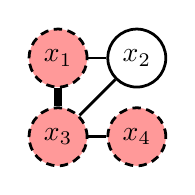
\begin{tikzpicture}[line width=1pt,node distance=14mm ,main/.style = {draw, circle},scale=1] 
   \node[main,fill=red!40!white,densely dashed] at (0,1) (x1) {\texttt{$x_1$}};
   \node[main,color=black] at (1,1) (x2) {\texttt{$x_2$}};
       \node[main,fill=red!40!white,densely dashed] at (0,0) (x3) {\texttt{$x_3$}};
       \node[main,fill=red!40!white,densely dashed] at (1,0) (x4) {\texttt{$x_4$}};
      \draw (x1) -- (x2);
       \draw [line width = 3pt, color=black] (x1) -- (x3);
      \draw (x2) -- (x3);
      \draw (x3) -- (x4);
   \end{tikzpicture}
   };
   
       \draw [decorate,decoration={brace,amplitude=10}] (0,2.5) -- (6,2.5) node [black,midway,xshift=-0.6cm] {};
   
       %\node[text width=6cm] at (2,-2){$\DP[i,c]$};
       %\node[text width=6cm] at (5.5,-2){$\DP[i,c+\{x_4\to \texttt{gray/dotted}]$};
      
   \end{tikzpicture}
   }}
% \end{figure}


%In order to derive the above recurrence relation, let $F$ be a matching from the set $\RP(b,M)$. Note that $v \notin M$, as $M \subseteq X_b$. Therefore, $v$ will be matched by some edge $uv \in F$. Now there are two possible cases: either $u \notin X_b$ or $u \in X_b$. For the former case when $u \notin X_b$, it is clear that there is a bijection between all such matchings $F$ and all elements of $\RP(c,M)$. Therefore, number of such matchings correspond to the first term $\pma[c,M]$ of the recurrence relation. Now let us consider the latter case when $u \in X_b$, then the matching $F \setminus uv \in \RP(c,M M \cup \{u, v\})$, and number of such matchings correspond to the second term $\sum_{u \in X_b\setminus M:\ uv\in E(G)}\pma[c, M \cup \{v,u\}]$ of the recurrence relation.
%




% To prove that consider any $(X_b, M)$-respectful matching $F$. Since $v \notin M$, $v$ should be matched with some point, say, $u$. Then if $u\notin X_b$, matching $F$ is $(X_{c}, M)$-respectful, and number of such cases corresponds to the first term. If $u \in X_b$ then mathching $F \setminus uv$ is $(X_{c}, M \cup \{u, v\})$ respectful and correspondence is one-to-one.  

%This transition to $X_b$ can be computed in $\bigO(\lvert X_b\rvert) = \bigO(\pw(G))$ time.
\end{compactitem}


\begin{proposition}[Proof in~\ref{app:proof}]\label{prop:comp_pw_perfmat}
	
	Given a graph $G$ with $n$ vertices and a nice path decomposition $\mathcal{P} $ of $G$ with $O(n)$ bags and width $\pw,$ the algorithm above finds the total number of perfect matchings/Kekulé structures in time $\bigO(n\cdot \poly(\pw) \cdot2^{\pw}).$
	
%The time complexity for finding the total number of perfect matchings for a graph $G = (V,E)$, with $\lvert V \rvert = n$ and pathwidth $\pw$, using the above algorithm is .
% The final complexity is $\bigO(n\cdot \textup{pw}\cdot2^{\textup{pw}})$
\end{proposition}


%\subsubsection{Bounded Treewidth}\label{subsec:perfect_treewidth}
%We now present a dynamic programming approach over the nice tree decomposition of the given graph $G$. The definitions of respectful perfect matchings and dynamic programming states used here are same as Section \ref{subsec:perfect_pathwidth}. Let $\mathcal{T} = \{T, \{X_t\}_{t \in V(T)}\}$ be a nice tree decomposition of the graph $G = (V,E)$ under consideration.

% We will use a dynamic programming over the nice tree decomposition. Definitions of dynamic programming and respectfulness have only cosmetic differences with path decomposition case. Let us fix a nice tree decomposition $\mathcal{T} = \{T, \{X_t\}_{t \in V(T)}\}$. For each $b \in T$ and each $M \subseteq X_b$ we will define $\dpt[b, M]$ as a number of perfect matchings in a $G_b^\downarrow \setminus M$ such that each matching edge $uv$ has at least on point in $G_b^\downarrow \setminus X_b$: $u \notin X_b$ or $v \notin X_b$. We call such matchings \textit{respectful} to the $(X_b, M)$.


% \begin{remark}

% \end{remark}
% If $X_l = \varnothing$ is a leaf bag, we have only empty $(X_l, \varnothing)$-respectful matching, which means 
% \[
% 	\dpt[X_l, \varnothing] = 1.
% \]

% Also for the root bag $X_r$, $\dpt[X_r, \varnothing]$ contains number of perfect matchings in a whole graph $G$.


% Cases of introduce and forget nodes repet verbatim. We need only consider merge case now. 
%We now provide a bottom-up approach for filling up the dynamic table. As mentioned earlier, the dynamic table relations depend on the type of the bag. There are now four possible cases for the type of bags, i.e., when $X_b$ is: leaf node, introduce node, forget node and join node respectively. The reccurrence relations for leaf node, introduce node and forget node remains the same as Section \ref{subsec:perfect_pathwidth}. Therefore, we only need to consider the case of join node which is described as follows:

\paragraph{Extension to Tree Decompositions} We now extend our algorithm above to handle tree decompositions. Assume that the input includes a nice tree decomposition $\mathcal{T} = \{T, \{X_t\}_{t \in V(T)}\}$ of the graph $G$ with width $\twi.$ As before, we perform a bottom-up dynamic programming and treat leaves and introduce/forget nodes exactly as in the previous algorithm. Computations at join nodes are performed as follows:
\begin{compactitem}
	\item \textbf{Join Nodes:} Let $b$ be a join node with children $c_1$ and $c_2.$ We have:
\[
\textstyle \pma[b,M] = \sum_{H_1 \sqcup H_2 = X_b \setminus M}\pma[c_1,M\cup H_2]\cdot \pma[c_2, M\cup H_1].
% \\
% &=\sum_{H \subseteq X_b \setminus M}\pma[c_1,M\cup H]\cdot \pma[c_2, X_b \setminus H],\\
\]

where $H_1 \sqcup H_2 = X_b \setminus M$ means $H_1 \cup H_2 = X_b \setminus M$ and $H_1 \cap H_2 = \emptyset.$ 
% This two formulas yields same result, but first easier to analyze and second easier to implement.  
In order to derive the above recurrence relation, let $F$ be a matching from the set $\RP(b,M)$. By Lemma~\ref{joinseplemma}, $F$ does not have any edges between $G_{c_1}^\downarrow \setminus X_b$ and $G_{c_2}^\downarrow \setminus X_b$. Therefore, it can be split into two matchings, $F_1 := E(G_{c_1}^\downarrow) \cap F$ and $F_2 := E(G_{c_2}^\downarrow) \cap F$. Let $H_1 := V(F_1) \cap X_b$ and $H_2 := V(F_2) \cap X_b$. Based on Definition~\ref{def:respectful_perfect_matching}, we have $F_1 \in \RP(c_1,M \cup H_2)$ and $F_2 \in \RP(c_2,M \cup H_1)$. If we choose $H_1$ and $H_2$ such that $H_1 \sqcup H_2 = X_b \setminus M$, then for all such matchings $F_1 \in \RP(c_1,M\cup H_2)$ and $F_2 \in \RP(c_2, M\cup H_1)$, we get a matching $ F = F_1 \cup F_2$, such that $F \in \RP(b,M).$ %This leads to our recurrence relation.


% \begin{figure}[h]
% \floatbox[{\capbeside\thisfloatsetup{capbesideposition={right,top},capbesidewidth=5cm}}]{figure}[\FBwidth]
% {\caption{Computing the values at join nodes. Bag $b$ has children $c_1$ and $c_2$. Nodes $x_3$ and $x_4$ have been matched with elements not in $b$, but these elements could have been in the subtree of $c_1$ or the subtree of $c_2$. We thus iterate over all possible ways to distribute these matched nodes between $c_1$ and $c_2$. For each of these ways, we multiply the number of respectful matchings in $c_1$ and $c_2$, then, finally, we add these results together to find the answer for $b$.
% }\label{fig:join_node}}
% {\resizebox{0.6\textwidth}{!}{% !TEX root = ../main.tex
\begin{tikzpicture}[line width=1pt,node distance=14mm ,main/.style = {draw, rectangle},scale=1] 

    \node[scale=.8] at (-4,1){$\textup{PerfMatch}[b,\{x_1,x_4\}]$};
       \node[main] at (-4,-0.5) (9) {
   \begin{tikzpicture}[line width=1pt,node distance=14mm ,main/.style = {draw, circle},scale=1] 
   \node[main,fill=red!40!white,densely dashed] at (0,1) (x1) {\texttt{$x_1$}};
   \node[main,color=black] at (1,1) (x2) {\texttt{$x_2$}};
       \node[main,color=black] at (0,0) (x3) {\texttt{$x_3$}};
       \node[main,fill=red!40!white,densely dashed] at (1,0) (x4) {\texttt{$x_4$}};
      \draw  (x1) -- (x2);
       \draw (x1) -- (x3);
      \draw (x2) -- (x3);
      \draw (x3) -- (x4);
   \end{tikzpicture}
       };
       
    \node[scale=.8] at (0,5.5){$\textup{PerfMatch}[c_1,\{x_1,x_4\}\cup \{x_2,x_3\}]$};
       \node[main] at (0,4) (8) {
   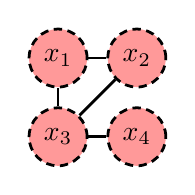
\begin{tikzpicture}[line width=1pt,node distance=14mm ,main/.style = {draw, circle},scale=1] 
   \node[main,fill=red!40!white,densely dashed] at (0,1) (x1) {\texttt{$x_1$}};
   \node[main,fill=red!40!white,densely dashed] at (1,1) (x2) {\texttt{$x_2$}};
       \node[main,fill=red!40!white,densely dashed] at (0,0) (x3) {\texttt{$x_3$}};
       \node[main,fill=red!40!white,densely dashed] at (1,0) (x4) {\texttt{$x_4$}};
      \draw (x1) -- (x2);
       \draw (x1) -- (x3);
      \draw (x2) -- (x3);
      \draw (x3) -- (x4);
   \end{tikzpicture}
   };
   
    \node[scale=3] at (2,4){$\cdot$};
   
    \node[scale=.8] at (4,5.5){$\textup{PerfMatch}[c_2,\{x_1,x_4\}\cup \{\}]$};
   \node[main] at (4,4) (8) {
   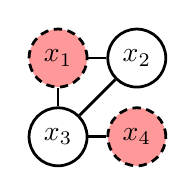
\begin{tikzpicture}[line width=1pt,node distance=14mm ,main/.style = {draw, circle},scale=1] 
   \node[main,fill=red!40!white,densely dashed] at (0,1) (x1) {\texttt{$x_1$}};
   \node[main,color=black] at (1,1) (x2) {\texttt{$x_2$}};
       \node[main,color=black] at (0,0) (x3) {\texttt{$x_3$}};
       \node[main,fill=red!40!white,densely dashed] at (1,0) (x4) {\texttt{$x_4$}};
      \draw (x1) -- (x2);
       \draw (x1) -- (x3);
      \draw (x2) -- (x3);
      \draw (x3) -- (x4);
   \end{tikzpicture}
   };
   
    \node[scale=.8] at (0,2.5){$\textup{PerfMatch}[c_1,\{x_1,x_4\}\cup \{x_3\}]$};
   \node[main] at (0,1) (8) {
   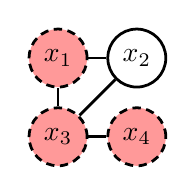
\begin{tikzpicture}[line width=1pt,node distance=14mm ,main/.style = {draw, circle},scale=1] 
   \node[main,fill=red!40!white,densely dashed] at (0,1) (x1) {\texttt{$x_1$}};
   \node[main,color=black] at (1,1) (x2) {\texttt{$x_2$}};
       \node[main,fill=red!40!white,densely dashed] at (0,0) (x3) {\texttt{$x_3$}};
       \node[main,fill=red!40!white,densely dashed] at (1,0) (x4) {\texttt{$x_4$}};
      \draw (x1) -- (x2);
       \draw (x1) -- (x3);
      \draw (x2) -- (x3);
      \draw (x3) -- (x4);
   \end{tikzpicture}
   };
   
    \node[scale=3] at (2,1){$\cdot$};
   
    \node[scale=.8] at (4,2.5){$\textup{PerfMatch}[c_2,\{x_1,x_4\}\cup \{x_2\}]$};
   \node[main] at (4,1) (8) {
   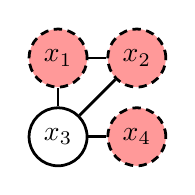
\begin{tikzpicture}[line width=1pt,node distance=14mm ,main/.style = {draw, circle},scale=1] 
   \node[main,fill=red!40!white,densely dashed] at (0,1) (x1) {\texttt{$x_1$}};
   \node[main,fill=red!40!white,densely dashed] at (1,1) (x2) {\texttt{$x_2$}};
       \node[main,color=black] at (0,0) (x3) {\texttt{$x_3$}};
       \node[main,fill=red!40!white,densely dashed] at (1,0) (x4) {\texttt{$x_4$}};
      \draw (x1) -- (x2);
       \draw (x1) -- (x3);
      \draw (x2) -- (x3);
      \draw (x3) -- (x4);
   \end{tikzpicture}
   };
   
    \node[scale=.8] at (0,-0.5){$\textup{PerfMatch}[c_1,\{x_1,x_4\}\cup \{x_2\}]$};
   \node[main] at (0,-2) (8) {
   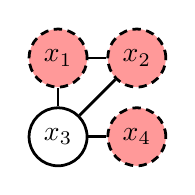
\begin{tikzpicture}[line width=1pt,node distance=14mm ,main/.style = {draw, circle},scale=1] 
   \node[main,fill=red!40!white,densely dashed] at (0,1) (x1) {\texttt{$x_1$}};
   \node[main,fill=red!40!white,densely dashed] at (1,1) (x2) {\texttt{$x_2$}};
       \node[main,color=black] at (0,0) (x3) {\texttt{$x_3$}};
       \node[main,fill=red!40!white,densely dashed] at (1,0) (x4) {\texttt{$x_4$}};
      \draw (x1) -- (x2);
       \draw (x1) -- (x3);
      \draw (x2) -- (x3);
      \draw (x3) -- (x4);
   \end{tikzpicture}
   };
   
    \node[scale=3] at (2,-2){$\cdot$};
   
    \node[scale=.8] at (4,-0.5){$\textup{PerfMatch}[c_2,\{x_1,x_4\}\cup \{x_3\}]$};
   \node[main] at (4,-2) (8) {
   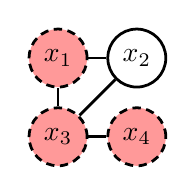
\begin{tikzpicture}[line width=1pt,node distance=14mm ,main/.style = {draw, circle},scale=1] 
   \node[main,fill=red!40!white,densely dashed] at (0,1) (x1) {\texttt{$x_1$}};
   \node[main,color=black] at (1,1) (x2) {\texttt{$x_2$}};
       \node[main,fill=red!40!white,densely dashed] at (0,0) (x3) {\texttt{$x_3$}};
       \node[main,fill=red!40!white,densely dashed] at (1,0) (x4) {\texttt{$x_4$}};
      \draw (x1) -- (x2);
       \draw (x1) -- (x3);
      \draw (x2) -- (x3);
      \draw (x3) -- (x4);
   \end{tikzpicture}
   };
   
    \node[scale=.8] at (0,-3.5){$\textup{PerfMatch}[c_1,\{x_1,x_4\}\cup \{\}]$};
   \node[main] at (0,-5) (8) {
   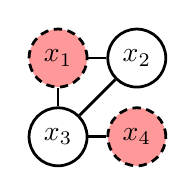
\begin{tikzpicture}[line width=1pt,node distance=14mm ,main/.style = {draw, circle},scale=1] 
   \node[main,fill=red!40!white,densely dashed] at (0,1) (x1) {\texttt{$x_1$}};
   \node[main,color=black] at (1,1) (x2) {\texttt{$x_2$}};
       \node[main,color=black] at (0,0) (x3) {\texttt{$x_3$}};
       \node[main,fill=red!40!white,densely dashed] at (1,0) (x4) {\texttt{$x_4$}};
      \draw (x1) -- (x2);
       \draw (x1) -- (x3);
      \draw (x2) -- (x3);
      \draw (x3) -- (x4);
   \end{tikzpicture}
   };
   
    \node[scale=3] at (2,-5){$\cdot$};
   
     \node[scale=.8] at (4,-3.5){$\textup{PerfMatch}[c_2,\{x_1,x_4\}\cup \{x_2,x_3\}]$};
   \node[main] at (4,-5) (8) {
   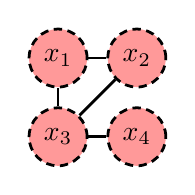
\begin{tikzpicture}[line width=1pt,node distance=14mm ,main/.style = {draw, circle},scale=1] 
   \node[main,fill=red!40!white,densely dashed] at (0,1) (x1) {\texttt{$x_1$}};
   \node[main,fill=red!40!white,densely dashed] at (1,1) (x2) {\texttt{$x_2$}};
       \node[main,fill=red!40!white,densely dashed] at (0,0) (x3) {\texttt{$x_3$}};
       \node[main,fill=red!40!white,densely dashed] at (1,0) (x4) {\texttt{$x_4$}};
      \draw (x1) -- (x2);
       \draw (x1) -- (x3);
      \draw (x2) -- (x3);
      \draw (x3) -- (x4);
   \end{tikzpicture}
   };
   
       \draw [decorate,decoration={brace,amplitude=10}] (-2,-5) -- (-2,4) node [black,midway,xshift=-0.6cm] {};
   
       %\draw [->](-2,3.5) -- (-3,2.5);
       %\draw [->](-2,1) -- (-3,0.5);
       %\draw [->](-2,-2) -- (-3,-1.5);
       %\draw [->](-2,-4.5) -- (-3,-3.5);
       %\draw [->](3.5,-2.5) -- (5,-3);
       %\draw [->](3.5,-5) -- (5,-4.5);
       %\draw [->](3.5,-7.5) -- (5,-6);
       %\node[text width=6cm] at (2,-2){$\DP[i,c]$};
       %\node[text width=6cm] at (5.5,-2){$\DP[i,c+\{x_4\to \texttt{gray/dotted}]$};
      
   \end{tikzpicture}}}
% \end{figure}


% Consider arbitrary $(X_b, M)$-respectful matching $F$. By lemma \ref{joinseplemma} $F$ do not have edges between $G_{c_1}^\downarrow \setminus X_b$ and $G_{c_2}^\downarrow \setminus X_b$. Let us split this matching $F$ into $F_1 := E(G_{c_1}^\downarrow) \cap F$, $F_2 := E(G_{c_2}^\downarrow) \cap F$, also let $H_1 := V(F_1) \cap X_b$, $H_2 := V(F_2) \cap X_b$. Observe that $F_1$ is $(X_{c_1}, M \cup H_2)$-respectful and $F_2$ is $(X_{c_2}, M \cup H_1)$-respectful. Notice that if $H_1, H_2$ are chosen, $F_1, F_2$ acts independently, so when $H_1, H_2$ fixed such matching could be counted as $\dpt[c_1, M \cup H_2] \cdot \dpt[c_2, M \cup H_1]$, which leads to our formula. 

\end{compactitem}

\begin{proposition}[Proof in~\ref{app:proof}]\label{prop:comp_tw_perfmat}
	
	
	Given a graph $G$ with $n$ vertices and a nice tree decomposition $\mathcal{T}$ of $G$ with $O(n)$ bags and width $\twi,$ the algorithm above finds the total number of perfect matchings/Kekulé structures in time $\bigO(n\cdot \poly(\twi)\cdot3^{\twi})$.
\end{proposition}

% Figures illustrating the dynamic programming algorithm are provided in Appendix~\ref{appendix:figure_perfect_matching}.


\subsection{Merrifield--Simmons Index / Counting Independent Sets}\label{sec:independent_sets}

% Our approach for counting independent sets is very similar to the case of matchings.

\begin{definition}[Respectful Independent Sets]\label{def:respectful_independent_sets}
Let $\mathcal{P} = \{X_1, \dots X_r\}$ be a nice path decomposition of $G.$ For each bag $b$ and each $M \subseteq X_b$, we define $\RI(b,M)$ as the set of all independent sets $I$ in a $G_b^\downarrow $ such that $I \cap X_b = M$, and $\ind[b, M]$ as the size of this set.
\end{definition}


\paragraph{Our Dynamic Programming Algorithm} Since $X_r = \emptyset$ is the root node, $G_{r}^\downarrow = G$, and all independent sets of $G$ are counted by $\ind [r, \emptyset].$ As in previous cases, our algorithm is a bottom-up dynamic programming that processes each bag according to its type:
\begin{compactitem}
\item \textbf{Leaf Nodes:} If $X_l$ is a leaf bag then $\RI(l,M)$ contains only the empty independent set as $X_l = \emptyset$. Therefore, $\ind[l,\emptyset]=1$.
\item \textbf{Introduce Nodes:} Let $b$ be an introduce bag with child $c$ and $X_b = X_c \cup \{v\}$. We have: 
\[
\ind [b,M] =
\begin{cases}
\ind [c,M] &v \notin M\\
\ind [c,M\setminus v] &v \in M \textup{ and } N(v) \cap M = \emptyset \\
0 &v \in M \textup{ and } N(v) \cap M \neq \emptyset
\end{cases}
\]
In the first case, $v$ is not meant to be in the independent set, thus we can simply look into independent sets conforming to the same $M$ in $c.$ The second case is similar, except that $v$ is in the independent set. However, note that all neighbors of $v$ in $G^\downarrow_b$ are in $X_b.$ Thus, it suffices to check whether any neighbor of $v$ is included in the independent set inside the current bag. The final case is when the set $M$ is invalid and picking neighbors.

%In order to derive the above recurrence relations, we have to consider two possibilities for $v$.
%\begin{enumerate}
%\item If $v \in M$, now there are again two subcases to consider i.e., $N(v)\cap M \ne \varnothing$ and $N(v)\cap M = \varnothing$. For the former subcase, there is a one-to-one correspondence with all such independent sets $I$ with elements of the set $\RI(c,M\setminus v)$. Therefore, $\ind[b,M] = \ind[c,M\setminus v]$ for this subcase. For the latter subcase, there cannot exist any independent set $I$ in $\RI(b,M)$, such that it contains both $v$ and its neighbours. Therefore, $\ind[b,M] = 0$ for this subcase. 

%% then by Definition \ref{def:respectful_independent_sets}, all the elements of the set $\RI(b,M)$ are in one-to-one correspondence with all the elements of the set $\RP(c, M \setminus v)$. 
%\item If $v \notin M$, then there is a bijection between $\RI(b,M)$ and $\RI(c,M)$. Therefore, number of indepedent sets $\ind[b,M]$ is equal to $\ind[c,M]$. 
%\end{enumerate}
%This transition from $X_c$ to $X_b$ can be computed in $\bigO(1)$ time. 
\item \textbf{Forget Nodes:} Let $b$ be a forget node such that $X_b = X_c \setminus \{v\}$. We have $
\ind [b,M] = \ind[c,M] + \ind[c,M\cup \{v\}].$
Since $X_b \subseteq X_c,$ we know that $G^\downarrow_b = G^\downarrow_c.$ Thus, we simply need to check the two possibilities for the intersection of the independent set with $G^\downarrow_c,$ based on whether it includes or excludes $v.$

%In order to derive the above recurrence relation, let $I$ be an independent set from the set $\RI(b,M)$. Now there are two possible cases i.e., either $v \notin I$ or $v \in I$. For the former case when $v \notin I$, there is a bijection for all such independent sets $I$ to all the elements of the set $\RI(c,M)$. Therefore, number of such independent sets is equal to $\ind[c,M]$, and this corresponds to the first term of the recurrence relation. For the latter case when $v \in I$, there is a bijection between all such independent sets $I$ to all the elements of the set $\RI[c,M\cup \{v\}]$. Therefore, number of such independent sets is equal to $\ind[c,M\cup \{v\}]$, which is the second term of the recurrence relation.
%
%This transition to $X_b$ can be computed in $\bigO(1)$ time.
\end{compactitem}



\begin{proposition}\label{prop:comp_pw_ind}
	
		Given a graph $G$ with $n$ vertices and a nice path decomposition $\mathcal{P} $ of $G$ with $O(n)$ bags and width $\pw,$ the algorithm above finds the Merrifield--Simmons  index, i.e.~the total number of independent sets, in time $\bigO(n\cdot \poly(\pw) \cdot2^{\pw}).$
		
%The time complexity for finding the total number of independent sets for a graph $G = (V,E)$, with $\lvert V \rvert = n$ and pathwidth $\pw$, using the above algorithm is $\bigO(n\cdot \poly(\pw) \cdot2^{\pw})$.
% The final complexity is $\bigO(n\cdot \textup{pw}\cdot2^{\textup{pw}})$
\end{proposition}
%\begin{proof}
%	The runtime analysis is identical to Proposition \ref{prop:comp_pw_perfmat}.
%%Proof same as Proposition \ref{prop:comp_pw_perfmat}.
%% For each bag, we have atmost $2^{\pw}$ dynamic programming states, and for each state we spend atmost $\bigO(\poly(\pw))$ time. It is known that there are atmost $\bigO(n)$ bags for any nice path decomposition of $G$ \cite[Chapter 7]{cygan2015parameterized}. Therefore, we spend atmost $\bigO(n\cdot \poly(\pw) \cdot2^{\pw})$ time to completely fill the dymamic programming table.
%\end{proof}

\begin{comment}
\subsubsection{Bounded Treewidth}\label{sec:tw_indep}
% We will use a dynamic programming approach over the nice tree decomposition of the given graph $G$. The definitions of respectful matchings and dynamic programming states used here are same as Section \ref{sec:pw_indep}. Let $\mathcal{T} = \{T, \{X_t\}_{t \in V(T)}\}$ be a nice tree decomposition of the graph $G = (V,E)$ under consideration.

Before we procced with the dynamic progamming algorithm, we first prove the following technical lemma which will be required for the derivation of recurrence relations. 
\begin{lemma}\label{lem:technical_lemma_ind_join_node}
Let $X_b$ be the join node with $X_{c_1}$ and $X_{c_2}$ as its children, then $\lvert \RI(b,M)\rvert  = \lvert \RI(c_1,M) \rvert \cdot \lvert \RI(c_2,M) \rvert$.
\end{lemma}

\begin{proof}
Let $f$ be the map from $\RI(b,M)$ to $\RI(c_1,M) \times \RI(c_2,M)$ such that $f$ is defined as follows:

\[
	f(I) \mapsto (I_1,I_2)
\]
where $I_1 = I \cap V(G_{c_1}^\downarrow)$ and $I_2 = I \cap V(G_{c_2}^\downarrow)$ then we will show that $f$ is a bijection.

First, we will show that $f$ is injective. Let $I,J \in \RI(b,M)$ such that $f(I) = f(J)$, then we need to show that $I = J$. Let us assume that $I \ne J$, this implies that there exists $u \in I$, such that $u \notin J$. As $f(I) = f(J)$, we get $(I_1,I_2) = (J_1,J_2)$, this implies $I = J$, as $I = I_1 \cup I_2$ and $J = J_1 \cup J_2$. Therefore, we get a contradiction to our initial assumption that $I \ne J$, this implies that $f$ is injective.

Now, we will show that $f$ is surjective. Let $(J,K) \in \RI(c_1,M) \times \RI(c_2,M)$ then we need to show that there exists an $I \in \RI(b,M)$ such that $f(I) = (J,K)$. Let $I$ be $J \cup K$. In order to complete the proof, we need to show that $I \in \RI(b,M)$ and $f(I) = (J,K)$. For all $u,v \in I$, we need to show that there doesn't exist any edge between $u$ and $v$. We need to consider the following cases for $u$ and $v$:
\begin{itemize}
	\item $u,v \in J$ or $u,v \in K$: In both the cases, there doesn't exist any edge between $u$ and $v$ as both $J$ and $K$ are independent sets of $G_{c_1}^\downarrow$ and $G_{c_2}^\downarrow$ respectively.
	\item $u \in J \setminus J \cap K$ and $v \in K \setminus J \cap K$: We know using Lemma \ref{joinseplemma}, that there is no edge between $V(G_{c_1}^\downarrow) \setminus X_b$ and $V(G_{c_2}^\downarrow) \setminus X_b$. Therefore, there is no edge between $u$ and $v$.
\end{itemize}
This completes the proof that $I$ is an independent set of $G_{b}^\downarrow$. As $I = J \cup K$ and $J\cap X_b = K \cap X_b = M$, this implies that $I \cap X_b = M$. Therefore, this completes the proof that $I \in \RI(b,M)$ and shows that $f$ is a surjective map.
\end{proof}

% We now provide a bottom-up approach for filling up the dynamic table. The dynamic table relations depend on the type of the bag. There are four possible cases for the type of bags, i.e., when $X_b$ is: leaf node, introduce node, forget node and join node respectively. 
The reccurrence relations for leaf node, introduce node and forget node remains the same as Section \ref{sec:pw_indep}. Therefore, we only need to consider the case of join node which is described as follows:
\end{comment}

\begin{compactitem}
	\item \textbf{Join Nodes:} Let $b$ be a join node with ${c_1}$ and ${c_2}$ as its children. We have
	$
	\ind[b,M] = \ind[c_1,M] \cdot \ind[c_2,M]
	$
	This is because $M$ fixes exactly which vertices in $X_b$ are to be included in the independent set. Moreover, Lemma~\ref{joinseplemma} guarantees that only the vertices in $X_b$ are shared between $G^\downarrow_{c_1}$ and $G^\downarrow_{c_2}.$ Therefore, every independent set $I_b \in \RI(b, M)$ of $G^\downarrow_b$ is the union of a unique combination of an independent set $I_{c_1} \in \RI(c_1, M)$ of $G^\downarrow_{c_1}$ and another independent set $I_{c_2} \in \RI(c_2, M)$ of $G^\downarrow_{c_2}.$
%This recurrence relation follows from Definition \ref{def:dp_indpendent_set} and Lemma \ref{lem:technical_lemma_ind_join_node}.
\end{compactitem}
%This transition to $X_b$ can be computed in $\bigO(1)$ time.


\begin{proposition}\label{prop:ind_tw_match}
Given a graph $G$ with $n$ vertices and a nice tree decomposition $\mathcal{T} $ of $G$ with $O(n)$ bags and width $\twi,$ the algorithm above finds the Merrifield--Simmons  index, i.e.~the total number of independent sets, in time $\bigO(n\cdot \poly(\twi) \cdot2^{\twi}).$
\end{proposition}
%\begin{proof}
%	The runtime analysis is identical to Proposition \ref{prop:comp_pw_perfmat}.
%\end{proof}

\todo{add figures for all cases above}

%\subsection{Matchins and Independent Sets of All Sizes}\label{sec:matchings_indep_sets_all_sizes}
%Due to space constraints, we added this section to the 
% \subsection{Counting Matchings of All Sizes}\label{sec:entropy_matchings}

% In this section, given a graph $G$ and a tree/path decomposition, our goal is to find the number of matchings of size $k$ in $G$ for every $k.$
% We need to only slightly adapt the dynamic programming values defined in Section~\ref{sec:matchings}, in order to count matchings of each size separately. The derivation of recurrence relations and their correctness is also very similar to Section~\ref{sec:matchings}. Finally, given this information, computing the entropy is a simple matter of applying Equation~\eqref{eq:entropy}.



% \begin{definition}[Respectful Matchings of size $k$]\label{def:respectful_matching_size_k}
% Given a nice path decomposition $\mathcal{P} = \{X_1, \dots X_r\}$ of $G,$ for each bag $b$ and each $M \subseteq X_b$, we define $\RM(b,k,M)$ as the set of all matchings $F$ in  $G_b^\downarrow \setminus M$ such that (i)~$\lvert F \rvert = k$; (ii)~each matching edge $uv \in F$ has at least one endpoint in $G_b^\downarrow \setminus X_b$; and (iii)~every vertex in $X_b \setminus M$ is covered by $F$. We further define $\ma[b,k,M] := |\RM(b,k,M)|.$
% \end{definition}

% \paragraph{Our Dynamic Programming Algorithm} Since $X_r = \emptyset$ is the root node, $G_{r}^\downarrow = G$, and $\ma [r, k,\varnothing]$ counts matchings of size $k$ in $G$. We process the bags in a bottom-up order as follows:
% % If $X_l = \varnothing$ is a leaf bag, only $(X_l, \varnothing)$-respectful matching is an empty 
% % matching, which means: 
% % \[
% % \dpt[X_l, \varnothing] = 1.
% % \]


% % We now provide a bottom-up approach for filling up the dynamic table. The dynamic table relations depend on the type of the bag. We need to consider three cases when $X_b$ is: leaf node, introduce node and forget node respectively.
% \begin{compactitem}
% \item \textbf{Leaf Nodes:} If $X_l$ is a leaf bag then $\RM(l,k,M)$ contains only the empty matching as $X_l = \emptyset$. Therefore, $\ma[l,0,\emptyset] = 1$ and for any other $k > 0$ $\ma[l,k,\emptyset] = 0$.
% \item \textbf{Introduce Nodes:} If $b$ introduces $v$ and has a single child $c$ then, we have:
% \[
% \ma [b,k,M] =
% \begin{cases}
% \ma [c,k,M\setminus v] &v \in M\\
% 0 &v \not\in M
% \end{cases}.
% \]

% \item \textbf{Forget Nodes:} Let $b$ be a forget node with child $c$ and $X_b = X_c \setminus \{v\}$, then
% \[
% \ma[b,k,M]= \ma[c,k,M] +  \ma[c,k,M \cup \{v\}] 
% + \sum_{u \in X_b\setminus M:\ uv\in E(G)}\ma[c,k-1, M \cup \{u, v\}].
% \]

% \end{compactitem}

% \begin{proposition}\label{prop:comp_pw_matchings_size_k} \label{prop:twe}
	
% 		Given a graph $G$ with $n$ vertices and a nice path decomposition $\mathcal{P} $ of $G$ with $O(n)$ bags and width $\pw,$ the algorithm above finds the number of matchings of size $k$ for every $0 \leq k \leq \frac{n}{2}$ in time $\bigO(n^2 \cdot \poly(\pw) \cdot2^{\pw}).$
	
% %The time complexity for finding the total number of matchings of all possible sizes for a graph $G = (V,E)$, with $\lvert V \rvert = n$ and pathwidth $\pw$, using the above algorithm is $\bigO(n^2\cdot \poly(\pw) \cdot2^{\pw})$.
% %% The final complexity is $\bigO(n\cdot \textup{pw}\cdot2^{\textup{pw}})$
% \end{proposition}
% \begin{proof}
% The analysis is similar to that of Proposition~\ref{prop:comp_pw_perfmat}, except that we now have $O(n)$ times as many dynamic programming values, one for each value of $k.$
% \end{proof}
% %\subsubsection{Bounded Treewidth}\label{sec:entropy_matchings_tw}
% % We will use a dynamic programming approach over the nice tree decomposition of the given graph $G$. The definitions of respectful matchings of fixed size and dynamic programming states used here are same as Section \ref{sec:entropy_matchings_pw}. Let $\mathcal{T} = \{T, \{X_t\}_{t \in V(T)}\}$ be a nice tree decomposition of the graph $G = (V,E)$ under consideration.

% %% We now provide a bottom-up approach for filling up the dynamic table. The dynamic table relations depend on the type of the bag. There are four possible cases for the type of bags, i.e., when $X_b$ is: leaf node, introduce node, forget node and join node respectively. 
% %The reccurrence relations for leaf node, introduce node and forget node remains the same as Section \ref{sec:entropy_matchings_pw}. Therefore, we only need to consider the case of join node which is described as follows:

% \paragraph{Extension to Tree Decompositions} 
% If the input contains a tree decomposition rather than a path decomposition, our algorithm proceeds in a bottom-up order and handles the join nodes as follows:
% \begin{compactitem}
% 	\item \textbf{Join Nodes:} 
% 	Let $b$ be a join node with children ${c_1}$ and ${c_2}.$ We define $n_b := \lvert V(G_b^{\downarrow}) \rvert$. We define $n_{c_1}$ and $n_{c_2}$ similarly and, without loss of generality, assume that $n_{c_1} \leq n_{c_2}$\footnote{If $n_{c_1} = n_{c_2}$ we choose the lexicographically smaller bag as $c_1.$}. We call $c_1$ the \emph{light} child of $b$ and $c_2$ the \emph{heavy} child. We also note that 
% 	\begin{equation} \label{eq:oneandhalf} n_b = n_{c_1} + n_{c_2} - |X_b| \geq 2 \cdot n_{c_1} - |X_b|.
% \end{equation}
% Finally, we have:
% \begin{equation} \label{eq:joinmatch}
% \hspace{-1cm}\ma[b,k,M] = 
% \sum_{0\leq k_{1}\leq \frac{n_{c_1}}{2}} \sum_{H_1 \sqcup H_2 = X_b \setminus M}\ma[c_1,k_{c_1},M\cup H_2]\cdot \ma[c_2,k-k_1, M\cup H_1].
% \end{equation}
% \end{compactitem}
% This is similar to Section~\ref{sec:matchings}, except that we choose to explicitly keep track of the number of matching edges that come from $G^\downarrow_{c_1},$ i.e.~$k_1,$ and the other $k-k_1$ edges of the matching come from $G^\downarrow_{c_2}.$ Note that the first sum above is on $n_{c_1}$ where $c_1$ was the light child of $b.$



% %\begin{lemma}\label{lem:technical_lemma_for_matching_entropy}
% %Let $\mathcal{T} = \{T, \{X_t\}_{t \in V(T)}\}$ be a nice tree decomposition of the graph $G = (V,E)$. Then $\sum n_a$ for all smaller subtrees $T_a$ in $\SSt(\mathcal{T})$ is at most $\bigO(n\cdot \log n)$.
% %
% %% Then $ \sum_{T_a \in \SSt(\mathcal{T})} n_a$ is atmost $\bigO(n\cdot log(n))$.
% %\end{lemma}
% %\begin{proof}
% %Let $x_v$ be the number of times any vertex $v$ appears in the smallest subtree of some node with more than one child.
% %
% %\[\sum_{T_a \in \SSt(\mathcal{T})}n_a = \sum_{v\in T} x_v \]
% %
% %Observe that $v$ can have at most $\log n$ ancestors with degree more than two in which it is part of the smallest subtree.
% %
% %This can be shown by keeping track of the current subtree and iterating through the ancestors of $v$. Every time $v$ is in the smallest subtree of a node with more than one child, the size of such subtree doubles, and this can happen at most $\log n$ times.
% %
% %Therefore, we get the following bound on number of vertices for all smaller subtrees:
% %\[
% %\sum_{T_a \in \SSt(\mathcal{T})}n_a = \sum_{v\in T} x_v \leq \sum_{v\in T} \log n \leq n \log n
% %\]
% %\end{proof}

% % \begin{figure}[h]
% % \resizebox{0.32\textwidth}{!}{% !TEX root = ../main.tex
% \begin{center}
\begin{tikzpicture}[node distance={17mm}, thick, main/.style = {draw, rectangle split,rectangle split parts=2}] 
\node[main] (0) []{ $n_b = 72$ \nodepart{two}$x_1,x_2,x_3$}; 
\node[main] (00) [below left of =0]{ $n_b = 40$ \nodepart{two}$x_1,x_2,x_3$};
\node[] (000) [below of =00,node distance={8mm}]{...};

\node[main,fill=cyan!20, dashed] (01) [below right of =0]{$n_b = 35$ \nodepart{two}$x_1,x_2,x_3$};
\node[] (010) [below of =01,node distance={8mm}]{...};
\node[main] (011) [below of =010,node distance={8mm}]{$n_b = 29$ \nodepart{two}$x_1,x_{10},x_{11}$};
\node[main] (0110) [below left of =011]{$n_b = 20$ \nodepart{two}$x_1,x_{10},x_{11}$};
\node[] (0110p) [below of =0110,node distance={8mm}]{...};
\node[main,fill=cyan!20, dashed] (0111) [below right of =011]{$n_b = 12$ \nodepart{two}$x_1,x_{10},x_{11}$};
\node[] (0111p) [below of =0111,node distance={8mm}]{...};
\node[main] (01110) [below of =0111p,,node distance={8mm}]{$n_b = 6$ \nodepart{two}$x_{10},\textcolor{red}{x_{15}}$};
\node[] (01110p) [below of =01110,node distance={8mm}]{...};

\draw [] (0) -- (00); 
\draw [] (00) -- (000); 

\draw [line width=3pt] (0) -- (01); 
\draw [] (01) -- (010); 
\draw [] (010) -- (011); 

\draw [line width=3pt] (011) -- (0111); 
\draw [] (011) -- (0110); 
\draw [] (0110) -- (0110p); 

\draw [] (0111) -- (0111p); 
\draw [] (0111p) -- (01110); 

\draw [] (01110) -- (01110p); 


\end{tikzpicture}
% \end{center}}
% % \caption{This figure illustrates Proposition \ref{prop:comp_tw_matchings_size_k}. The tree shown represents a nice tree decomposition. Sequences of forget and introduce nodes have been omitted by ``...''. Bags in $L$, or bags that are the light child of some join bag, have been highlighted in blue (dashed). Notice that each of these bags has a parent $b$ with weight $n_b$ at least $1.5$ times the weight of its lightest child. Thus, a node, such as $x_{15}$, highlighted in red, can have at most $\log n$ light ancestors.
% % }
% % \label{fig:log_tree}

% % \end{figure}


% \begin{proposition}\label{prop:comp_tw_matchings_size_k}
	
% 		Given a graph $G$ with $n$ vertices and a nice tree decomposition $\mathcal{T}$ of $G$ with $O(n)$ bags and width $\twi,$ the algorithm above finds the number of matchings of size $k$ for every $0 \leq k \leq \frac{n}{2}$ in time $\bigO(n^2 \cdot \log n \cdot \poly(\twi) \cdot3^{\twi}).$
% %	
% %	
% %The time complexity for finding the total number of matchings of all possible sizes for a graph $G = (V,E)$, with $\lvert V \rvert = n$ and treewidth $\twi$, using the above algorithm is $\bigO(n^2 \cdot \log n  \cdot \poly(\twi)\cdot3^{\twi})$.
% %% With this, the final complexity of the algorithm increases to .
% \end{proposition}
% \begin{proof}
% 	Proof in \ref{appendix:proof_comp_tw_matchings_size_k}
	
% 	% All types of nodes except for join bags are covered by Proposition~\ref{prop:comp_pw_matchings_size_k}. Let $L$ be the set of all light children of join bags.
% 	% If $c \in L$ has a corresponding subgraph with size $n_c \leq 2 \cdot (\twi+1),$ then it will contribute only $\poly(\twi)$ iterations to the first sum in Equation~\eqref{prop:comp_tw_matchings_size_k}. Let $L' = \{c \in L : n_c > 2 \cdot (\twi + 1)\}.$
% 	% We claim that $\textstyle \sum_{c \in L'} n_c \in O(n \cdot \log n).$
% 	% The vertex $v$ will be counted in $n_c$ if and only if there is a descendant $d$ of $c$ that introduces $v.$ 
% 	% Consider any introduce bag $\eta$ and focus on the sequence $A_\eta$ of ancestors of $\eta$ in $T.$ The sizes of the subgraphs corresponding to the bags in this sequence are increasing as we move towards the root. If $c \in L' \cap A_\eta$ is an ancestor of $\eta$ that is also a light child of a join bag $b \in A_\eta,$ then, by Equation~\eqref{eq:oneandhalf} we have
% 	% $
% 	% n_b \geq 2 \cdot n_c - |X_b| \geq 2 \cdot n_c - (\twi + 1) \geq 1.5 \cdot n_c.
% 	% $
% 	% Thus, every time such a light ancestor is met, the size of the subgraph is multiplied by at least $1.5.$ Hence, $\eta$ can have at most $O(\log n)$ such ancestors. Since the tree decomposition has $O(n)$ bags and therefore $O(n)$ introduce bags $\eta$, each introducing a single vertex, which contributes to at most $O(\log n)$ terms of the sum, we have $\sum_{c \in L'} n_c \in O(n \cdot \log n).$ 
% 	% Finally, the total runtime of computing the sums of the form of Equation~\eqref{eq:joinmatch} is $O\left( \left(n \cdot \log n + n \cdot \poly(\twi)\right) \cdot n \cdot 3^{\twi}\right ).$ This is because we have $O(n)$ choices for $k$ and $O(3^\twi)$ choices for $M, H_1$ and $H_2$ as argued in Proposition~\ref{prop:comp_tw_perfmat}.
% \end{proof}


% \subsection{Counting Independent Sets of All Sizes}
% \label{sec:entropy_independent_sets}
% In this section, given a graph $G$ and a nice tree/path decomposition of $G$ as input, our goal is to find the number of independent sets of size $k$ in $G$ for every possible value of $k.$ As in the previous section, simply plugging these numbers into Equation~\eqref{eq:entropy} yields the entropy.

% % Similarly to the previous section, in this section we will introduce dynamic programming algorithms for computing independent sets of all sizes for the given graph $G$ for bounded pathwidth and bounded treewidth respectively. We need to slightly adapt the dynamic programming states defined in Section \ref{sec:independent_sets}, in order to count independent sets of all sizes. The derivation of the corresponding recurrence relations of dynamic programming states remain almost the same as Section \ref{sec:independent_sets}. So, we will provide proofs only for the cases which are significantly different from the earlier sections.

% %\subsubsection{Bounded Pathwidth}\label{sec:pw_indep_k} 

% \begin{definition}[Respectful Independent Sets of size $k$]
% \label{def:respectful_independent_sets_k}
% Let $\mathcal{P}$ be a nice path decomposition of $G$. For every bag $b$ and every $M \subseteq X_b$, we define $\RI(b,k,M)$ as the set of all independent sets $I$ in $G_b^\downarrow $ such that $I \cap X_b = M$ and $\lvert I \rvert=k$. We denote the size of this set as $\ind[b, k, M].$
% \end{definition}


% \paragraph{Our Dynamic Programming Algorithm} As in Section~\ref{sec:independent_sets}, $\ind [r, k, \emptyset]$ is the number of independent sets of size $k$ in $G$. We process our decomposition bottom-up as follows:
% \begin{compactitem}
% \item \textbf{Leaf Nodes:} If $X_l$ is a leaf bag then $\RI(l,k,M)$ contains only the empty independent set as $X_l = \emptyset$. Therefore, $\ind[l,0,\emptyset]=1$ and for any other $k > 0$ $\ind[l,k,\emptyset] = 0$.


% \item \textbf{Introduce Nodes:} Let $X_b$ be an introduce bag with $X_b = X_c \cup \{v\}$. We have:
% \[
% \ind [b,k,M] =
% \begin{cases}
% \ind [c,k,M] &v \notin M\\
% \ind [c,k-1,M\setminus v] &v \in M \textup{ and } N(v) \cap M = \varnothing \\
% 0 &v \in M \textup{ and } N(v) \cap M \neq \varnothing
% \end{cases}.
% \]
% \item \textbf{Forget Nodes:} Let $X_b$ be a forget node such that $X_b = X_c \setminus \{v\}$, then
% \[
% \textstyle \ind [b,k,M] = \ind[c,k,M] + \ind[c,k-1,M\cup \{v\}].
% \]
% \end{compactitem}



% \begin{proposition}\label{prop:comp_pw_ind_ent}
	
% 			Given a graph $G$ with $n$ vertices and a nice path decomposition $\mathcal{P} $ of $G$ with $O(n)$ bags and width $\pw,$ the algorithm above finds the number of independent sets of size $k$ for every $0 \leq k \leq n$ in time $\bigO(n^2 \cdot \poly(\pw) \cdot2^{\pw}).$
% 	\end{proposition}
% \begin{proof}
% The runtime analysis is identical to Proposition~\ref{prop:twe}.
% \end{proof}

% %\subsubsection{Bounded Treewidth}
% \label{sec:tw_indep_k}

% % We will use a dynamic programming approach over the nice tree decomposition of the given graph $G$. The definitions of respectful matchings and dynamic programming states used here are same as Section \ref{sec:pw_indep_k}. Let $\mathcal{T} = \{T, \{X_t\}_{t \in V(T)}\}$ be a nice tree decomposition of the graph $G = (V,E)$ under consideration.

% % We now provide a bottom-up approach for filling up the dynamic table. The dynamic table relations depend on the type of the bag. There are four possible cases for the type of bags, i.e., when $X_b$ is: leaf node, introduce node, forget node and join node respectively. 
% %The reccurrence relations for leaf node, introduce node and forget node remains the same as Section \ref{sec:pw_indep_k}. Therefore, we only need to consider the case of join node which is described as follows:

% \paragraph{Extension to Tree Decompositions} As in the previous cases, we only need to specify how the algorithm handles join nodes.
% \begin{compactitem}
% 	\item \textbf{Join Nodes:} Let $b$ be a join node with light child $c_1$ and heavy child $c_2.$ We have:
% 		\[ \textstyle
% 		\ind[b, k, M] = \sum_{0\leq k_1 \leq n_{c_1}} \ind[c_1,k_1, M] \cdot \ind[c_2,k-k_1+\vert M \vert,M].
% 	\]
% 	This is because every independent set $I \in \RI(b, k, M)$ of size $k$ in the graph $G^\downarrow_b$ can be uniquely written as the union of two independent sets $I_1$ of size $k_1$ in $\RI(c_1, k_1, M)$ and $I_2$ of size $k_2$ in $\RI(c_2, k_2, M).$ Since we have $I_1 \cap I_2 = M$ and $|I_1 \cup I_2| = k,$ we must have $k_2 = k - k_1 + |M|.$
% \end{compactitem}


% % Using \ref{def:smaller_subtree} to bound the sum of $n_{c_1}$ over all join nodes:



% \begin{proposition}\label{prop:comp_tw_independent_sets_size_k}
	
% 		Given a graph $G$ with $n$ vertices and a nice tree decomposition $\mathcal{T}$ of $G$ with $O(n)$ bags and width $\twi,$ the algorithm above finds the number of independent sets of size $k$ for every $0 \leq k \leq {n}$ in time $\bigO(n^2 \cdot \log n \cdot \poly(\twi) \cdot2^{\twi}).$
	
% \end{proposition}
% \begin{proof}
% The runtime analysis is similar to that of Proposition~\ref{prop:comp_tw_matchings_size_k}.
% \end{proof}

\todo{add figures for the 4 cases in all sections above}

